\documentclass[10pt]{beamer}\usepackage[]{graphicx}\usepackage[]{color}
%% maxwidth is the original width if it is less than linewidth
%% otherwise use linewidth (to make sure the graphics do not exceed the margin)
\makeatletter
\def\maxwidth{ %
  \ifdim\Gin@nat@width>\linewidth
    \linewidth
  \else
    \Gin@nat@width
  \fi
}
\makeatother

\definecolor{fgcolor}{rgb}{0.345, 0.345, 0.345}
\newcommand{\hlnum}[1]{\textcolor[rgb]{0.686,0.059,0.569}{#1}}%
\newcommand{\hlstr}[1]{\textcolor[rgb]{0.192,0.494,0.8}{#1}}%
\newcommand{\hlcom}[1]{\textcolor[rgb]{0.678,0.584,0.686}{\textit{#1}}}%
\newcommand{\hlopt}[1]{\textcolor[rgb]{0,0,0}{#1}}%
\newcommand{\hlstd}[1]{\textcolor[rgb]{0.345,0.345,0.345}{#1}}%
\newcommand{\hlkwa}[1]{\textcolor[rgb]{0.161,0.373,0.58}{\textbf{#1}}}%
\newcommand{\hlkwb}[1]{\textcolor[rgb]{0.69,0.353,0.396}{#1}}%
\newcommand{\hlkwc}[1]{\textcolor[rgb]{0.333,0.667,0.333}{#1}}%
\newcommand{\hlkwd}[1]{\textcolor[rgb]{0.737,0.353,0.396}{\textbf{#1}}}%

\usepackage{framed}
\makeatletter
\newenvironment{kframe}{%
 \def\at@end@of@kframe{}%
 \ifinner\ifhmode%
  \def\at@end@of@kframe{\end{minipage}}%
  \begin{minipage}{\columnwidth}%
 \fi\fi%
 \def\FrameCommand##1{\hskip\@totalleftmargin \hskip-\fboxsep
 \colorbox{shadecolor}{##1}\hskip-\fboxsep
     % There is no \\@totalrightmargin, so:
     \hskip-\linewidth \hskip-\@totalleftmargin \hskip\columnwidth}%
 \MakeFramed {\advance\hsize-\width
   \@totalleftmargin\z@ \linewidth\hsize
   \@setminipage}}%
 {\par\unskip\endMakeFramed%
 \at@end@of@kframe}
\makeatother

\definecolor{shadecolor}{rgb}{.97, .97, .97}
\definecolor{messagecolor}{rgb}{0, 0, 0}
\definecolor{warningcolor}{rgb}{1, 0, 1}
\definecolor{errorcolor}{rgb}{1, 0, 0}
\newenvironment{knitrout}{}{} % an empty environment to be redefined in TeX

\usepackage{alltt}
\usetheme{Warsaw}
\usepackage{graphicx}
\usepackage[utf8]{inputenc}
\usepackage{amsfonts}
\usepackage{amsmath}
\usepackage[notocbib]{apacite}
\usepackage{epstopdf}
\usepackage{booktabs}
\usepackage{colortbl, xcolor}

\setbeamertemplate{caption}{\centering\insertcaption\par}
\setlength{\belowcaptionskip}{15pt}
\renewcommand{\thetable}{}

\providecommand{\e}[1]{\ensuremath{\times 10^{#1}}}
\IfFileExists{upquote.sty}{\usepackage{upquote}}{}
\begin{document}


\date{}
\author{Micha\l{}  Burdukiewicz, Piotr Sobczyk}
\institute{ 
University of Wroc\l{}aw, Department of Genomics, Poland}

\title{Expanding signalHsmm using n-grams}


\begin{frame}
\maketitle





\end{frame}

\begin{frame}
\frametitle{Outline}
\tableofcontents
\end{frame}

\section{Motivation}


\begin{frame}
To improve our model, we added few supplementary states representing specific motives that might occur in the proximity of cleavage site. The structure of cleavage sites, more conserved than other parts of signal peptide, may be reflected by n-grams (k-mers), short vectors of $n$ characters derived from input sequences.
\end{frame}

\begin{frame}
\begin{figure}[ht]\centering

\includegraphics[scale=0.42]{HSMMs}
\caption{The diagram of simple (A) and extended version of signalHsmm with the n-gram cleavage site model (B).}
\label{fig:enccomp}
\end{figure}

\end{frame}


\AtBeginSection[]
{
\begin{frame}<beamer>
\frametitle{Outline}
\tableofcontents[currentsection]
\end{frame}
}

\section{Impact of the n-gram extension}

\begin{frame}

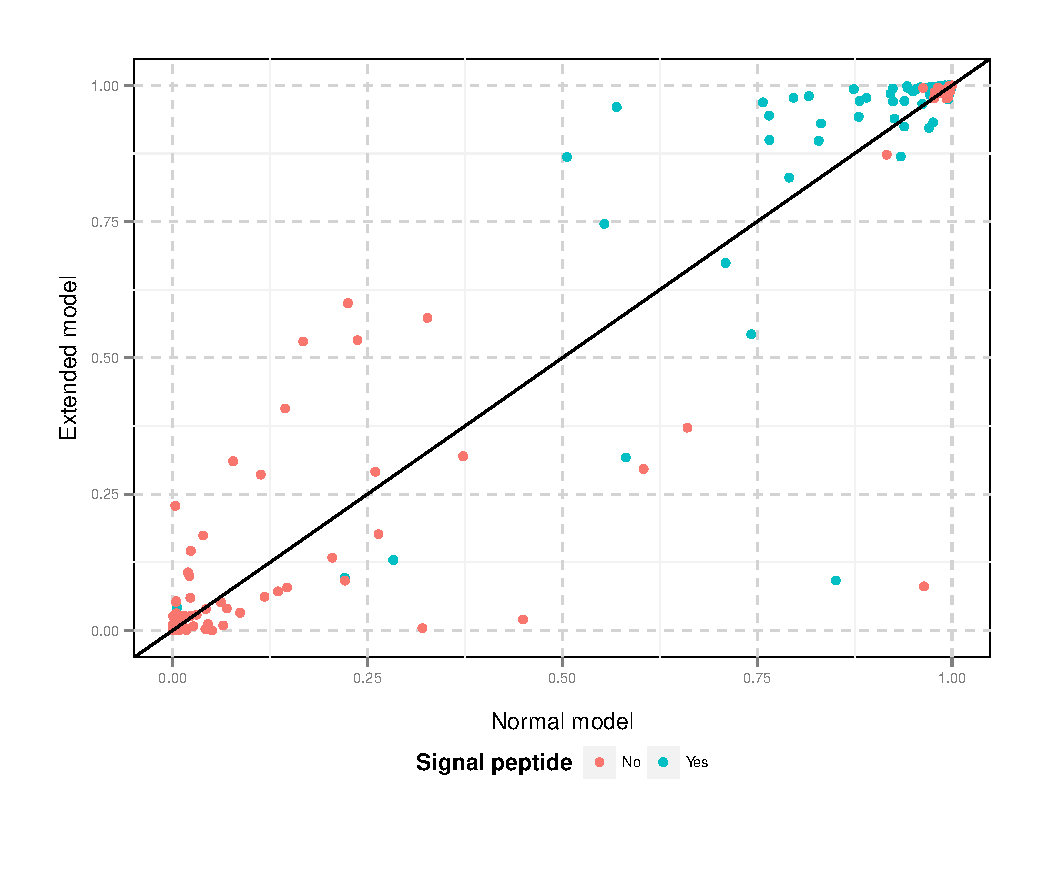
\includegraphics[width=\maxwidth]{figure/unnamed-chunk-2-1} 

\end{frame}

\begin{frame}
% latex table generated in R 3.2.1 by xtable 1.7-4 package
% Sun Jul 05 16:45:36 2015
\begin{table}[ht]
\centering
\caption{Performance of different classifiers.} 
\begin{tabular}{rrrrrr}
  \toprule
 & AUC & TP & TN & FP & FN \\ 
  \midrule
signalPnotm & 0.9416 &   208 &   195 &    19 &     6 \\ 
   \rowcolor[gray]{0.85}signalPtm & 0.9673 &   205 &   209 &     5 &     9 \\ 
  predsi & 0.8949 &   194 &   189 &    25 &    20 \\ 
   \rowcolor[gray]{0.85}phobius & 0.9509 &   207 &   200 &    14 &     7 \\ 
  philius & 0.9369 &   204 &   197 &    17 &    10 \\ 
   \rowcolor[gray]{0.85}signalHsmm2010 & 0.9526 &   198 &   191 &    23 &    16 \\ 
  signalHsmm1989 & 0.9562 &   202 &   194 &    20 &    12 \\ 
   \rowcolor[gray]{0.85}signalKmer & 0.9695 &   206 &   194 &    20 &     8 \\ 
   \bottomrule
\end{tabular}
\end{table}

\end{frame}







\section{Greedy n-gram choosing algorithm}

\begin{frame}
bla
\end{frame}



\end{document}
